\documentclass[journal]{IEEEtran} % use the `journal` option for ITherm conference style
\IEEEoverridecommandlockouts
% The preceding line is only needed to identify funding in the first footnote. If that is unneeded, please comment it out.
\usepackage{cite}
\usepackage{amsmath,amssymb,amsfonts}
\usepackage{algorithmic}
\usepackage{graphicx}
\usepackage{textcomp}
\usepackage{xcolor}
\usepackage{float}
\usepackage[justification=centering]{caption}
\raggedbottom

\def\BibTeX{{\rm B\kern-.05em{\sc i\kern-.025em b}\kern-.08em
    T\kern-.1667em\lower.7ex\hbox{E}\kern-.125emX}}
\newcommand{\imagewidth}{0.45\textwidth}
% \newcommand{\imageheight}{75mm}
\newcommand{\elvis}{\textit{Elvis}}
\begin{document}

\title{\elvis{}: A Highly Scalable Virtual Internet Simulator\\}

\author{%%%% author names
    \IEEEauthorblockN{Jacob Hollands},
    \IEEEauthorblockN{Mitchell Thompson},
    \IEEEauthorblockN{See-Mong Tan}
    \\%%%% author affiliations
    \IEEEauthorblockA{\textit{Western Washington University}}\\% first affiliation
    \IEEEauthorblockA{hollanj9, thomp288, see-mong.tan@wwu.edu}
}

\maketitle

\begin{abstract}
This research paper presents the development of a Network Description Language (NDL) in Rust for a simulation program called Elvis. The NDL creation involved the design and implementation of a new language, as well as a parser and generator to process the information. The language and accompanying tools were designed to allow users to easily create complex networks and machines for use in simulations. The NDL provides a straightforward way to define networks, applications, and machines, with an emphasis on flexibility and extensibility. The NDL was created with two core parts, a parser for converting the text to types and a generator to convert those types into an Elvis Simulation. The resulting NDL and tools provide a powerful framework for simulation programming and can be easily expanded upon for future use.

\end{abstract}

\begin{IEEEkeywords}
\elvis{}, NDL, Scalability, Networks
\end{IEEEkeywords}

\section{Introduction}
\elvis{} is a scalable simulation tool for a virtual Internet that is built using Rust. It differs from previous work in that high scalability is a primary goal of the simulation. In one experiment where all machines in the simulation continuously and concurrently send and receive data, we were able to scale up to 20,000 machines in a single simulation before memory limits were encountered. \elvis{} also provides ground-up, parallelizable constructions of key protocols including TCP/IP, DNS, and DHCP. rather than rely on existing OS implementations and virtualization technologies for isolation between machines. Instead, \elvis{} runs entirely in user space, vastly reducing both memory usage and overhead due to context switches.
Creating simulations within \elvis{} was initially challenging because users needed an in-depth understanding of \elvis{} and its core components to create networks and machines using Rust. Therefore, a Network Description Language (NDL) was developed to simplify the simulation creation process.

\section{Related Work}

In the realm of internet simulators, various approaches have been employed to describe simulations. For instance, SEEDEMU \cite{seedemu} adopts the usage of a Docker Compose file, which proves effective for simulators relying on Docker to establish distinct machines or networks. However, as Elvis operates in user space, this approach was not suitable. NS-3 \cite{ns3}, on the other hand, employs C++ for simulation creation. Nevertheless, we aim to steer clear of this approach due to its lack of scalability for larger simulations and usability for those who do not know C++.

\section{Design}
The design of the NDL was based on three criteria: simplicity, functionality, and scalability. The first criterion was simplicity, which was measured based on how easily users could translate their ideas into written descriptions using the language. User feedback and the team's usage of the language were analyzed to evaluate this criterion. The second criterion was the functionality of the NDL, which required a way to describe machines with networks, protocols, and applications, as well as a way to describe the networks the machines would operate on. Each of these subcategories had to be defined in the language, such as defining protocols for machines, for example, the UDP protocol. The third criterion was scalability, which required a robust language that did not need to be redefined every time a new feature was added.
We evaluated various available data description languages and originally decided to use JSON as the basis for the NDL. While it was successful in storing machines and networks with components such as protocols and applications, JSON did not meet the first criterion of simplicity because it required curly braces, square brackets, and colons to define objects. XML was also evaluated, but it still had some shortcomings, including the need for extensive formatting throughout the code, including the closing of each object with a closing tag. Therefore, it was decided to use a custom language that prioritized tabbing for its hierarchical structure, similar to how Python works, to make it more intuitive for users to read and write. The language also incorporated the square bracket notation, an extension from JSON’s curly brace formatting, for object definitions and a space-separated list of attributes for defining names and IDs.

\section{Syntax}
The NDL was designed to be simple, not only in its structure but also in its usage. In terms of core usage, the NDL consists of three main components: the core structure, the definitions, and the arguments.
\subsection{The Core Structure}
The NDL has a unique tabbing structure that helps to increase its simplicity over other languages. The structure is based on the number of tabs used for each sub-object or sub-definition of an object or definition. For example, if a Machine object is defined with internal components such as an Networks, Protocols, or other components, the internal components will be tabbed in one more time than the Machine was. The utilization of tabbing structure offers significant advantages such as maintaining relative positioning of each object and promoting clean code, particularly as simulations grow in size and more code is added.

\subsection{The Definitions}
The core definitions of the NDL are in two parts: Machines and Networks which can be seen in figure \ref{fig:basicsim}. The parser looks for these defining characteristics when computing the simulation. The [Networks] section refers to any and all Networks needed for the simulation. Similarly, the [Machines] section defines any and all Machines needed for the simulation. Additionally, either of those sections can be repeated if the user wants to break up their sections of code. It is worth noting that these sections, along with the [Protocols] and [Applications] sections seen in figure \ref{fig:basicsim}, are the only sections without extra arguments. This provides clarity in that these are defining sections, not information-providing sections.

\begin{figure}[H]
    \centerline{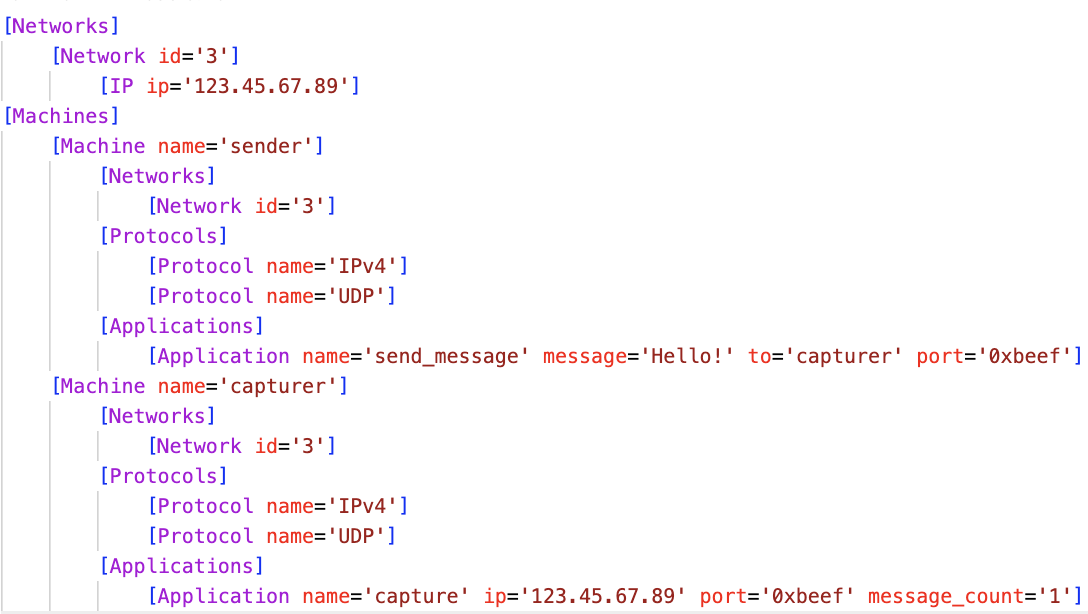
\includegraphics[width=\imagewidth]{Images/fig1.png}}
    \caption{Basic Simulation}
    \label{fig:basicsim}
\end{figure}


In a Networks section, one can list as many [Network] declarations as needed and inside each can provide either static IPs, or IP ranges for the Network. This can be seen in figure \ref{fig:corenetdef}. Similar to other sections of the NDL, one can declare as many IPs or IP ranges as needed and even can overlap IPs, however repeated IPs will be ignored.


\begin{figure}[H]
    \centerline{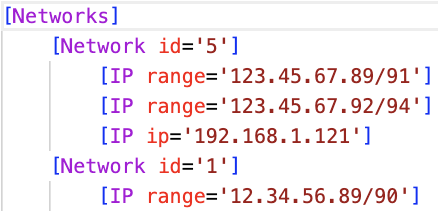
\includegraphics[width=\imagewidth]{Images/fig2.png}}
    \caption{Core Network Definitions}
    \label{fig:corenetdef}
\end{figure}

In the Machines section, there are three subsections: [Networks], [Applications], and [Protocols]. These sections have no arguments themselves and are defining sections. The [Networks] section is used to define the specific networks a machine is part of, allowing multiple machines to be on multiple different Networks. The [Protocols] section is used to define the specific protocols a machine uses, and the [Applications] section is used to define what a Machine does. The [Applications] section follows the same idea as the previous sections, allowing for multiple Applications and a variety of interchangeable arguments per each Application. This can be seen in figure \ref{fig:machinedef} where a full machine is defined.

\begin{figure}[H]
    \centerline{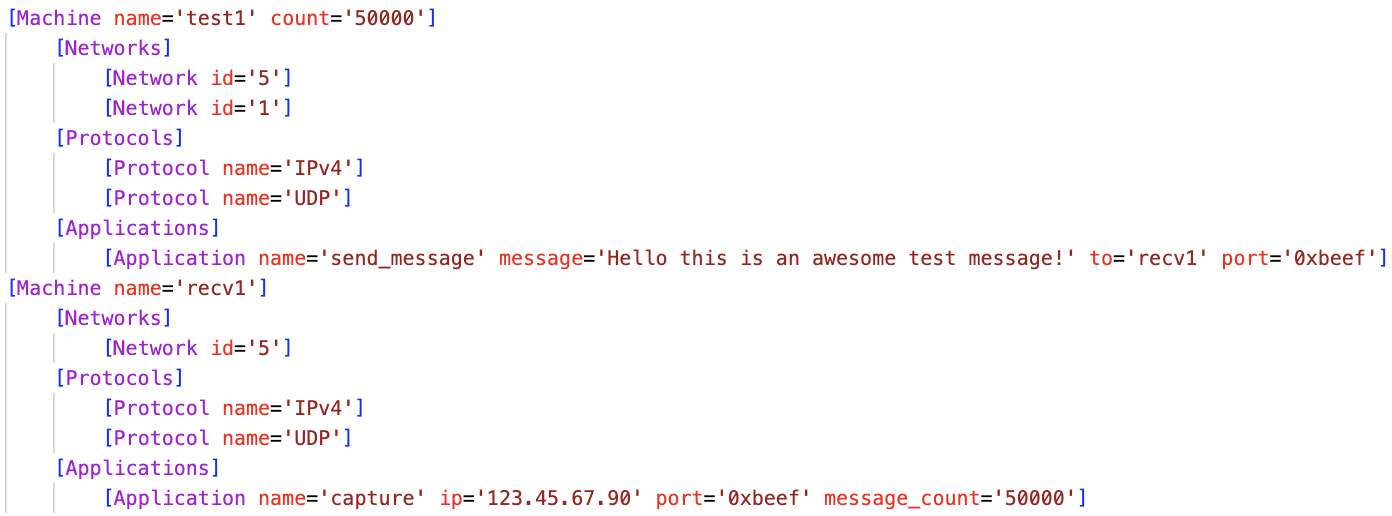
\includegraphics[width=\imagewidth]{Images/fig3.png}}
    \caption{Example Machine Definition}
    \label{fig:machinedef}
\end{figure}

\subsection{The Arguments}
The last core part of the NDL is how to provide the system with information. The core feature for providing information is through arguments. Arguments are defined through names and what those names are set to. For example, for an IP, one can provide either a range or ip argument and what it is equal to. This allows for easy definitions and the ability to stack arguments seamlessly, as the start and end quotes define each section. All definitions in the language follow this protocol, providing an easy entry point for using the NDL. An instance of this might appear as:
[IP range=’123.45.67.89/94’]
Or in the case of larger definitions such as for an application it may look similar to the following:

[Application name='send\_message' message='Hello this is an awesome test message!' to='recv1' port='0xbeef']

\section{Underlying Structure}
The underlying structure of the NDL was designed with scalability in mind. To ensure that changes to \elvis{} do not affect the parser's functionality, the NDL was separated into two main components.

\subsection{The Parser}
The parser's primary objective is to read the file's text and convert the data into various types that can be used later.
\subsubsection{Parser Structure}
The core structure of the parser has only a few steps involved. The first step is a general parser function that takes an entire section from an NDL file and parses it into the types described in the language. This function returns the type of the declaration, the parameters associated with it, and the remaining lines of the file after parsing that section. The general parser function is critical in creating an expandable language that can accommodate different declarations and parameters without having to edit the parser every time, which allows a declaration to have an effectively infinite number of parameters.

There are two additional functions besides the general parser function that are crucial to the NDL: the network parser and the machine parser. The network parser is in charge of parsing the [Networks] sections, while the machine parser handles the [Machines] sections. It is necessary to perform error checking with the various types to ensure that the right types are being utilized in the appropriate sections. For instance, only [Network] types should be permitted under a [Networks] type, and any other types will trigger an error.

\subsubsection{Data Types}
To ensure the effectiveness of the core parser structure, specific data types were required for translating text in the language into usable types in \elvis{}. Furthermore, to adapt to potential changes to \elvis{}, this range of distinct data types have been developed to cater to the various information requirements of simulations both presently and in the future.

The enumerator “DecType" contains the names of each different type, ranging from Networks to Applications. Using an enumerator was a sensible choice, as it allowed for easy comparisons between types without requiring string comparisons.

Simulations have two core components: a list of Networks and a list of Machines. The "Sim" type serves as a container for these core components, which both use HashMaps to allow for easy retrieval of data. Storing in HashMaps also provides the most flexibility in the future if new information or types are added.

Within any single component there can be a list of parameters, as discussed previously. Looking at the following example again: 

[Machine name='sender' count=’100']

The parameters are “name='sender' and count=’100'”. Since each of these parameters will be defined by a unique string, a HashMap with the key being “name” and “count” here with the values being string as well for everything within the single quotes. Having this type as a HashMap allows for looking up things such as the name, without having to loop through the entire list to find it.

The first core component of the parser, the [Network] type, requires three essential objects to be included: the "DecType", the parameters that need to be specified, and any defined IPs associated with it. To efficiently loop through the IPs during network generation, a Vector was chosen as the storage type due to its capacity to store and loop through a large number of elements. Within the IP type, the "DecType" and a list of "Params" are stored. This results in a fully functional and comprehensive [Networks] type that encompasses all necessary information for \elvis{}.
The second core component of the parser is the [Machine] type. This contains the "DecType," an optional list of parameters, the networks to which the machine belongs, the protocols it employs, and the applications it is running. The last three were separated into a separate type called "Interfaces" as the three together may be used in different scenarios.

Inside of “Interfaces” are the networks that the machine is on. The new types, “MachineNetworks” and “MachineNetwork,” were created here since they do not share the same characteristics as the previously discussed networks. “MachineNetwork” contains a “DecType” and the parameters the user inputs, while “MachineNetworks” is a Vector of “MachineNetwork”. The other two types, “Protocols” and “Applications”, share the exact same parameters, however, for the sake of readability and potential future expansion, they have been separated into different types. These types are formatted in exactly the same way, where they are Vectors of their respective type that contain the “DecType” and the list of parameters.

\subsubsection{Nom}
Nom is a community created Rust library. It provides a framework for defining parsers that can easily extract types, sections, and arguments from input data. With Nom, there is no need to manually match patterns in the data using text comparisons. Instead, the library's built-in functions make it easy to identify and extract the relevant information from the input. Nom was vital for the creation of the parser and its expandability.

\subsection{The Generator}
Once the parsing is complete, the parsed data needs to be transformed into Rust types that \elvis{} can understand. This is where the generator comes in. The generator is designed to accept any data type passed in from the parser section and translate it directly into \elvis-readable types. Valid \elvis{} types are generated so long as valid parsed data is passed to it.

\subsubsection{Core Structure}
Similar to the structure of the parser, the core structure of the generator relies on two main programs: a Network generator and a Machine generator. Networks must be generated first so that Machines can then use them.

\subsubsection{Translating Data Types}
Following the data types created for the parser, we now need to translate them into \elvis{}-readable data types. For the most part, this can be handled at translation time. Firstly, protocols can be directly translated into \elvis{} types, such that the generator reads in the arguments and creates an \elvis{} protocol which gets stored in a machine. However, the rest of the types such as networks are more complicated and require more processing. 
Specifically for networks, all of the information must be generated at once and stored in pieces that can later be used inside Machines or Applications. To accomplish this, the “NetworkInfo” structure was created, which can hold two main pieces of information: a HashMap of Network IDs, which machines can reference, and a HashMap of IDs to a Vector of IP addresses, which is needed because \elvis{} handles Networks based on IP tables correlated to specific Networks.
The remaining types from the parser do not need new generator types, but still require additional processing before being translated into \elvis{} types and are thus not direct translations.


\subsubsection{Network Generation}
The Network generator takes in the parsed Networks and returns the NetworkInfo structure previously referenced. This is the simplest part of the generator system, as it simply pulls the data from the parser and uses match statements to generate the specific parts of a network that \elvis{} needs. Essentially, it generates \elvis{} IPs from the strings provided, creating a Vector of IPs. It stores this in the previously mentioned manner and returns it to the core generator so that the Machines can then be generated.

\subsubsection{Machine Generation}
Machine generation is the more complicated side of generating. For each Machine specified in the language, a few operations must occur. First, it must check if the Machine has a count so that if the Machine needs to be generated multiple times, it can be. Then it must check if the Machine's name is specified. Alongside the name check, the most critical check that occurs here is the IP check. This checks if any of the given applications have IPs specified inside them. This allows the generator to pair a machine name with either the IP specified there or to the MAC address assigned to the machine. 

Following those checks, the \elvis{} machines begin to be generated and are stored into a Vector of machines. For each machine, it must generate an IP table specific to that machine given the networks it is a part of. Then, it checks which Protocols are specified, and finally which Applications are specified. IPs and Protocols are direct translation items, meaning that in the match statement for their string from the parser, they can simply be added to a Vector to be later compiled into the Machine. This direct translation looks something such as:

"IPv4" =\> protocols\_to\_be\_added.push(Ipv4::new(ip\_table
.clone()).shared())

For Applications, however, there are more checks specific to the arguments for each Application before direct translation can occur.

\subsubsection{Application Generator}

The Application Generator is a subset of the Machine generator. It is a collection of individual functions that take in the required arguments for an application and produce a compiled version of that application in \elvis{}. While the specific details of each function will vary depending on the application being generated, there are some core components that are present in each function. First, the function must ensure that all required arguments have been specified in the parse. For example, for the SendMessage application, this could include the message to be sent, as well as the IP or machine to which it will be sent. Next, the function must translate the specified arguments into valid \elvis{} types. If IP addresses or ports have been specified, they must be translated into a format that \elvis{} can understand. Additionally, if the application specifies a name in a particular field, the function must search the mapping to determine if that name corresponds to a valid IP or MAC address. Finally, once all of the compiled data has been generated, the function returns the compiled application to the machine generator for use.

This approach of using specific functions for each application makes it easy to expand the functionality of \elvis{} as new applications are added. When a user adds an application to \elvis{}, the generator can quickly translate the required information into the appropriate function. Additionally, in the future, these functions could be changed to macros, which would further simplify and generalize their use. With macros, users could simply specify the application to be returned and the information to be checked in the macro call, and the generator would dynamically check for that information.

Once applications have been generated, each machine is stored as a new machine in a Vector for use by \elvis{} during runtime. This process is repeated for all specified machines, and can be repeated multiple times if the machine has an associated count.

\section{Using The NDL}
The NDL can be utilized by invoking the \elvis{} executable with additional command line arguments. An example of a typical invocation of the program is as follows:

     ./elvis.exe --ndl ./simulations/basic/simulation.ndl
     
This instructs \elvis{} to perform the simulation specified in the file path. It is important to note that the file path can be either absolute or relative to the current working directory

\begin{figure}[H]
    \centerline{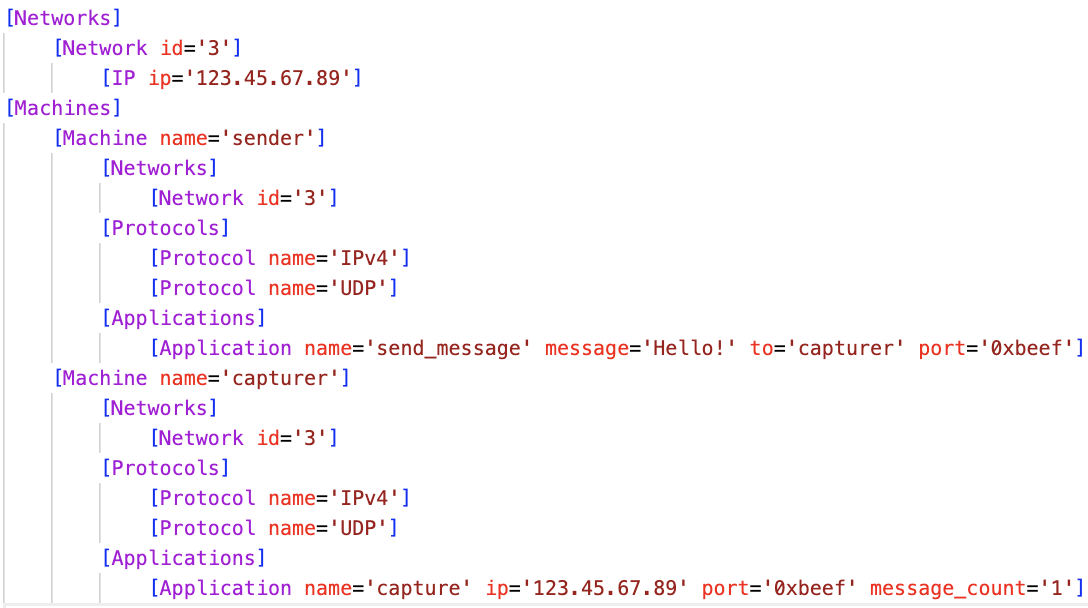
\includegraphics[width=\imagewidth]{Images/fig4.png}}
    \caption{A basic simulation with one machine sending a message to another}
    \label{fig:basicsim2}
\end{figure}

\begin{figure}[H]
    \centerline{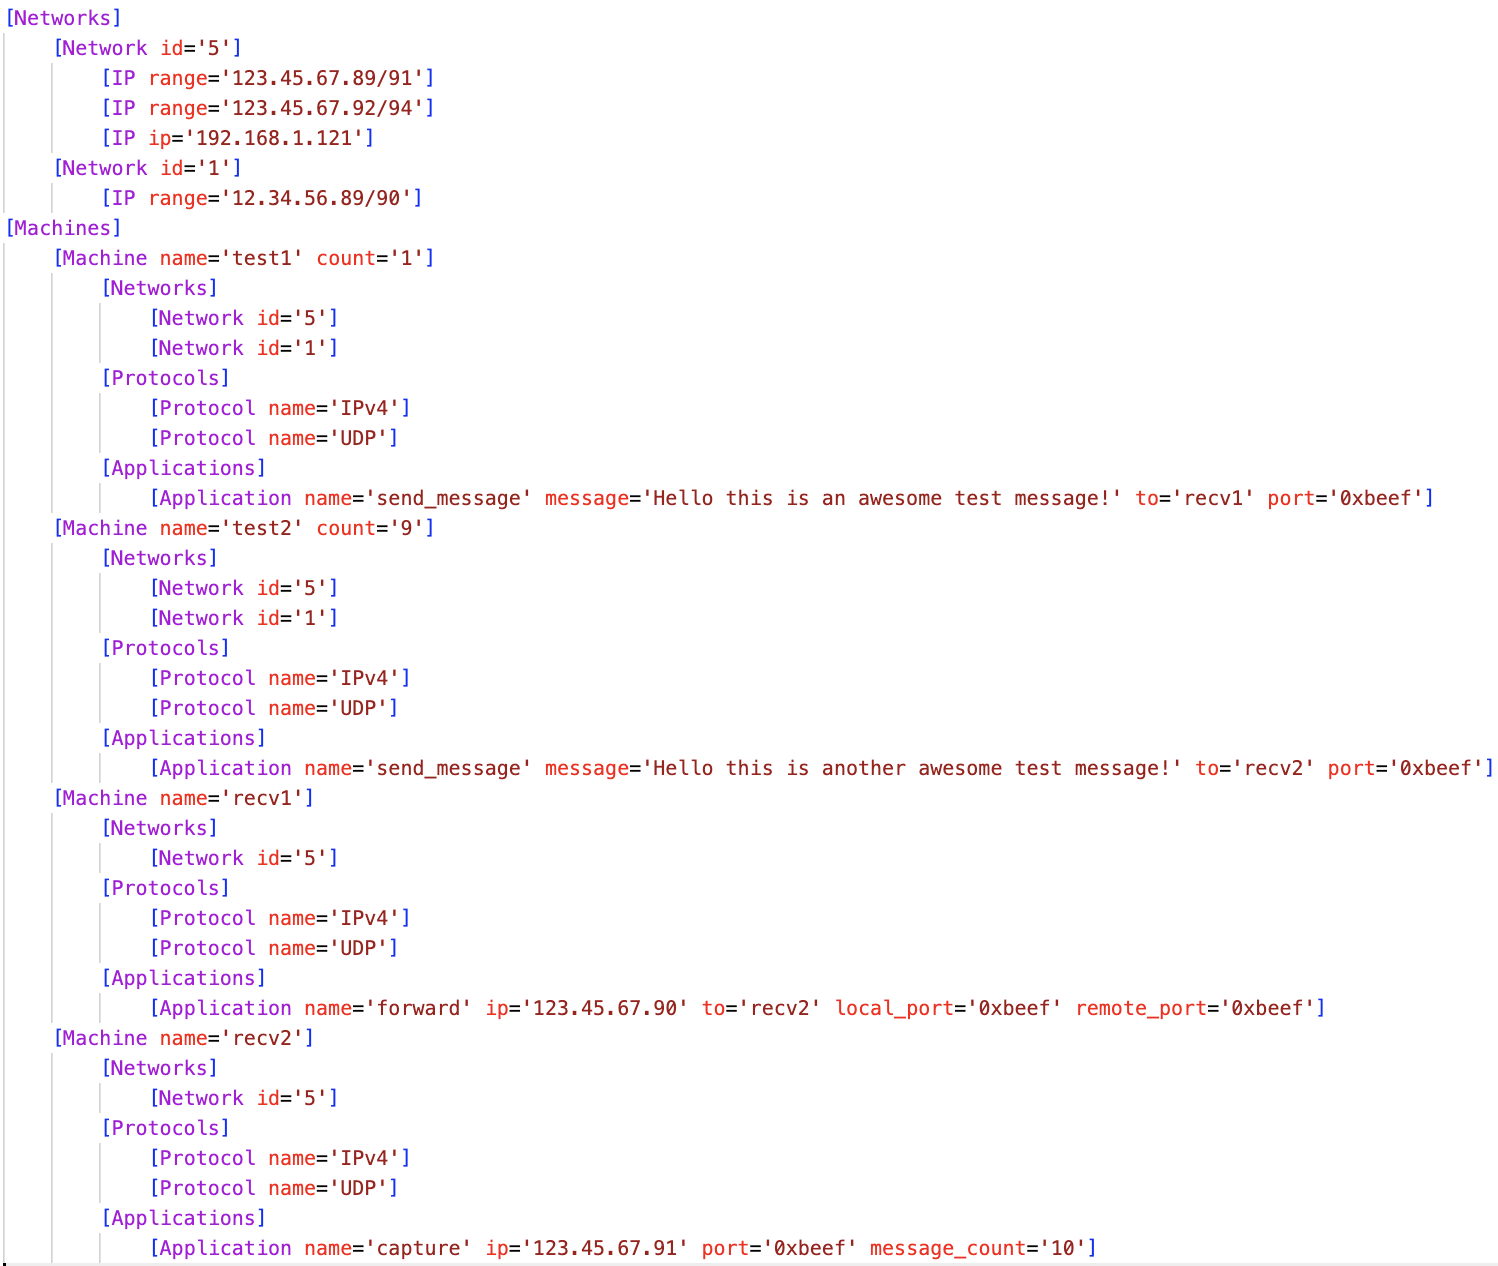
\includegraphics[width=\imagewidth]{Images/fig5.png}}
    \caption{A more complicated simulation with multiple machines sending messages to other machines}
    \label{fig:compsim}
\end{figure}

\begin{figure}[H]
    \centerline{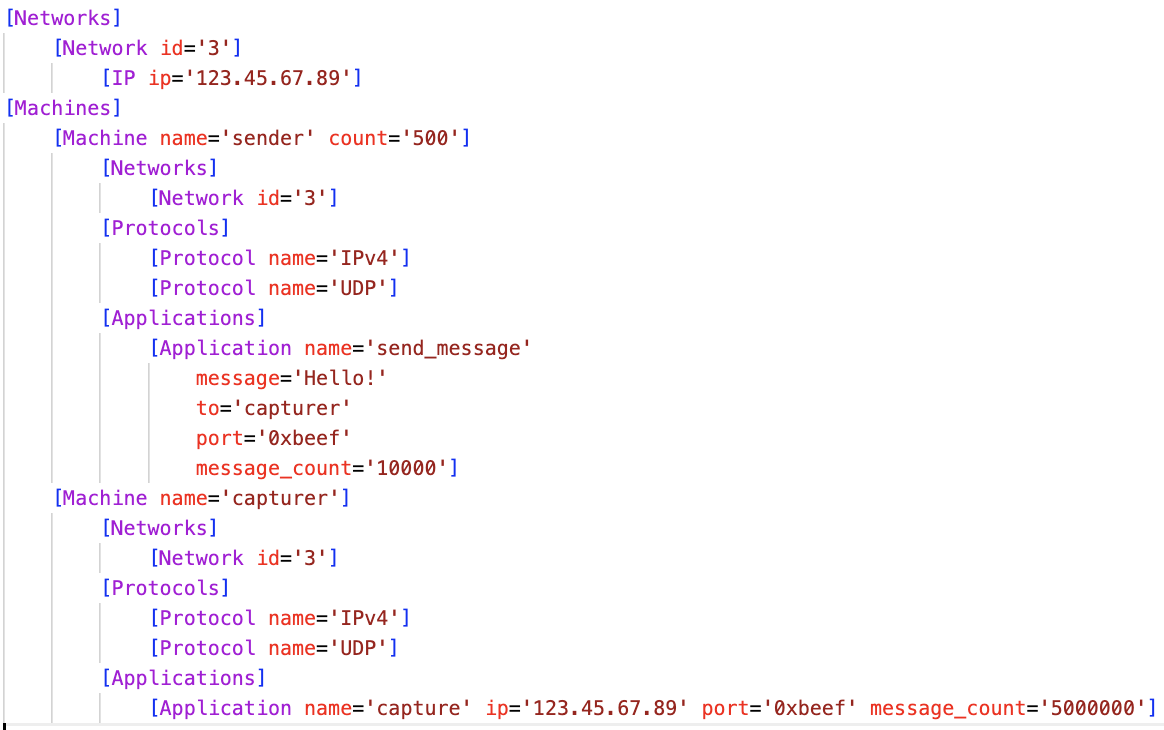
\includegraphics[width=\imagewidth]{Images/fig6.png}}
    \caption{A basic high-bandwidth simulation with 500 machines sending 10,000 messages each to one machine for a total of 5,000,000 messages}
    \label{fig:highband}
\end{figure}


\section{Conclusion}
The development of a Network Description Language in Rust for the simulation program \elvis{} has proven to be a successful undertaking. The creation of the NDL, along with the accompanying parser and generator, has provided a streamlined and efficient means of describing complex networks and machines for use in simulations. With the flexibility and expandability of the language and tools, future additions and modifications to \elvis{} can be easily accommodated. Overall, the development of this NDL has improved the functionality and usability of \elvis{}.



\begin{thebibliography}{00}
    \bibitem{rust} Klabnick, Steve and Nichols, Carol. 202. The Rust Programming Language. No Starch Press
    \bibitem{json} [1] M. Sporny, “JSON-LD 1.1,” W3C, https://www.w3.org/TR/json-ld11/
    \bibitem{xml} T. Bray, “Extensible Markup Language (XML),” Extensible markup language (XML) 1.0 (fifth edition), https://www.w3.org/TR/xml/ 
    \bibitem{seedemu} Zeng, Honghao, "Seedemu: The Seed Internet Emulator" (2021). Theses - ALL. 592. https://surface.syr.edu/thesis/592
    \bibitem{ns3} Riley, G.F., Henderson, T.R. (2010). The ns-3 Network Simulator. In: Wehrle, K., Güneş, M., Gross, J. (eds) Modeling and Tools for Network Simulation. Springer, Berlin, Heidelberg. https://doi.org/10.1007/978-3-642-12331-3\_2
    \bibitem{elvis} TBD



\end{thebibliography}



\section{Author Information}
Mitchell Thompson and Jacob Hollands are Masters candidates at Western Washington University. See-Mong Tan is an instructor at Western Washington University.

\end{document}
